\clearpage{\pagestyle{empty}\cleardoublepage}

\chapter{Multi-jet background estimation in the muon channel}\label{app:qcdmm}

We report in this appendix the method developed in year 2011 to better predict
the contribution from multi-jet background events in analyses with a single
muon and jets in the final state. 
For what concerns the studies presented in this appendix, data
from pp collisions at \cme\ of 7~\tev\ collected with the ATLAS
detector in 2011 are used, corresponding to a total integrated luminosity
of 689.5~\ipb. Details on the status of top analyses
using this dataset can be found in Reference~\cite{topCommonObjects2012}.
We refer to Section~\ref{sec:qcdbkg}
for the description of the general approach of the
Matrix Method and will present here the improvements we
made in the estimation by introducing a parametrization of
the $\epsilon_\mathrm{fake}$ as a function of the lepton
transverse momentum and of the minimum of the $\Delta R$ separation
between the muon and the jets,  min$\Delta R(\mu,j)$.
These parametrizations for the fake efficiencies 
are combined with the parametrization
in terms of muon pseudorapidity, which was used before.


The idea is that an increase in leading jet $p_T$ corresponds 
to higher hadronic activity nearby the lepton, 
which results in the fact that the event will no 
longer satisfy the tight selection requirement of 
isolation $\min\Delta R(\mu,j)>0.4$. This means a lower 
$\epsilon_\mathrm{fake}$. For the same reason we expect 
the fake efficiency to be lower for muons closer to jets.
We also expect these effects to increase with the number of 
jets in the event, a dependence that should be entering
in the $\epsilon_\mathrm{fake}$ parametrization as a function
of $\min\Delta R(\mu,j)$ (see Figure~\ref{fig:etaDep} and~\ref{fig:ljptmindrDep}). 

The muons are selected as ``tight'' if they pass the standard selection 
that was used in 2011 top analyses~\cite{topCommonObjects2012} 
(\texttt{combined} muons
passing {\tt EF$\_$mu18} trigger and track quality and isolation cuts,
summarized in Table~\ref{tab:tightloosemu}), while for the ``loose'' 
selections the requirements on calorimeter and tracker isolation
(\textit{etcone30}$<4~$GeV and \textit{ptcone30}$<4~$GeV respectively) 
are dropped.

\begin{table}[htb]\centering
\begin{tabular}{lcc}
cut & loose & tight \\\midrule
track ID quality cuts & $\checkmark$ & $\checkmark$\\
\texttt{combined} muon & $\checkmark$ & $\checkmark$\\
\texttt{tight} muon & $\checkmark$ & $\checkmark$\\
min$\Delta R(\mu,j)>0.4$ & $\checkmark$ & $\checkmark$\\
$e/\mu$ overlap removal& $\checkmark$ & $\checkmark$\\
\texttt{etcone30} $<4~$GeV &  & $\checkmark$\\
\texttt{ptcone30} $<4~$GeV &  & $\checkmark$\\\bottomrule
\end{tabular}
\caption{Selection cuts for tight and loose muons. The track ID quality cuts include
 $\pt(\mu) > 20 \GeV$ and $|\eta(\mu)| < 2.5$.}\label{tab:tightloosemu}
\end{table}

The efficiency $\epsilon_\mathrm{real}$ is estimated in a sample of $Z\rightarrow \mu\mu$ 
restricted to events with exactly 2 muons, one ``tight'' and one ``loose'' 
and requiring the dilepton reconstructed mass of the boson to be between 80-100~GeV. 
The control region to estimate $\epsilon_\mathrm{fake}$ is chosen as 
$5$~GeV$< E^{Miss}_T<15$~GeV in order to isolate a sample enriched 
in QCD, then the event is required to have a ``loose'' muon and at 
least one jet. Since contamination from muons from $W$ and $Z$ decays 
is still present in the low $E^{Miss}_T$ region, we try to achieve 
higher purity by correcting $N^{tight}$ and $N^{loose}$ as 
\begin{eqnarray}
N^{tight}_{corr} &&=  N^{tight} - N^{tight}_{W+jets,MC} - N^{tight}_{Z+jets,MC} - N^{tight}_{t\bar{t},MC}\\
N^{loose}_{corr} &&=  N^{loose} - N^{loose}_{W+jets,MC} - N^{loose}_{Z+jets,MC} - N^{loose}_{t\bar{t},MC}
\end{eqnarray}

Figure~\ref{fig:etaDep}~and~\ref{fig:ljptmindrDep}  
show $\epsilon_\mathrm{real}$ as a function of muon $\eta$ 
and  $\epsilon_\mathrm{fake}$ as a function of the variables 
on which we parametrize, i.e. muon $\eta$, leading jet $p_T$ 
and the minimum of $\Delta R(\mu,j)$.  The functions used don't 
have a specific physical meaning and are respectively 
\begin{equation}\label{eq:paruntagljpt}
f_{LJpT}(x) = p_0 + p_1/(x/100)^{p_2}
\end{equation} and 
\begin{equation}\label{eq:parmindr}
f_{min\Delta R}(x) = 0.5 p_0 (1+TMath::Erf( (x-p_1)/(\sqrt{2}p_2))).
\end{equation} 

If we add the requirement of having at least one tagged jet in 
the event, the $\epsilon_\mathrm{fake}$ efficiency changes (see Table~\ref{tab:averageeffs}). 
Efficiencies are computed in the same way as the untagged case 
but separately and requiring at least 1 \btag ged jet, where at the
time the \btag ging algorithm used was \texttt{SV0} with a weight cut 
of 5.85. While different $\epsilon_\mathrm{fake}$ where obtained in the
parametrizations with respect to lepton $\eta$ and jet \pt, 
no significant variations were observed in the dependency on
the minimum $\Delta R(\mu,j)$ and the pre-tag efficiencies are 
used in that case to exploit the higher statistics, like it's done for 
$\epsilon_\mathrm{real}$ where again the \btag ged events show 
no significant differences and more statistics 
for the estimation is available.

\begin{figure}\centering
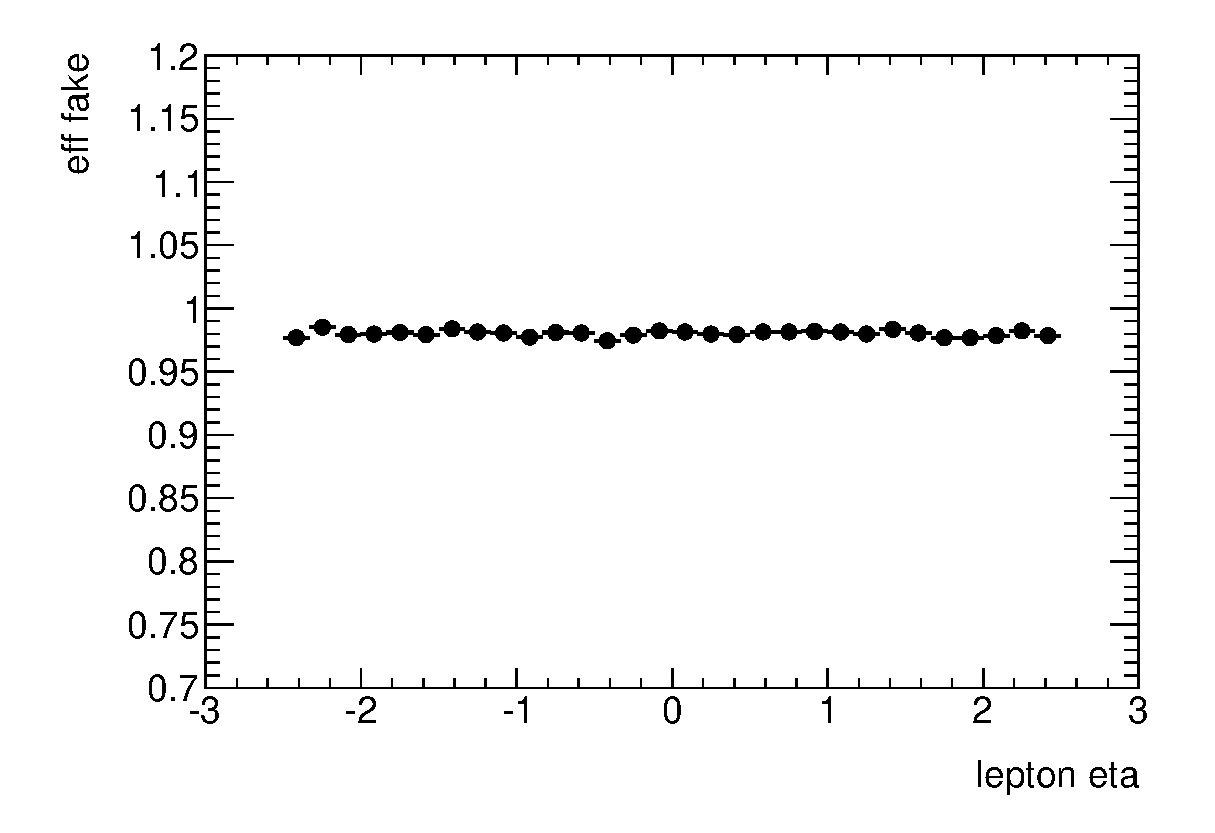
\includegraphics[width=.45\textwidth]{appendices/figures/mujets_mmB/fit_h_lep_eta_muon_real_untagged}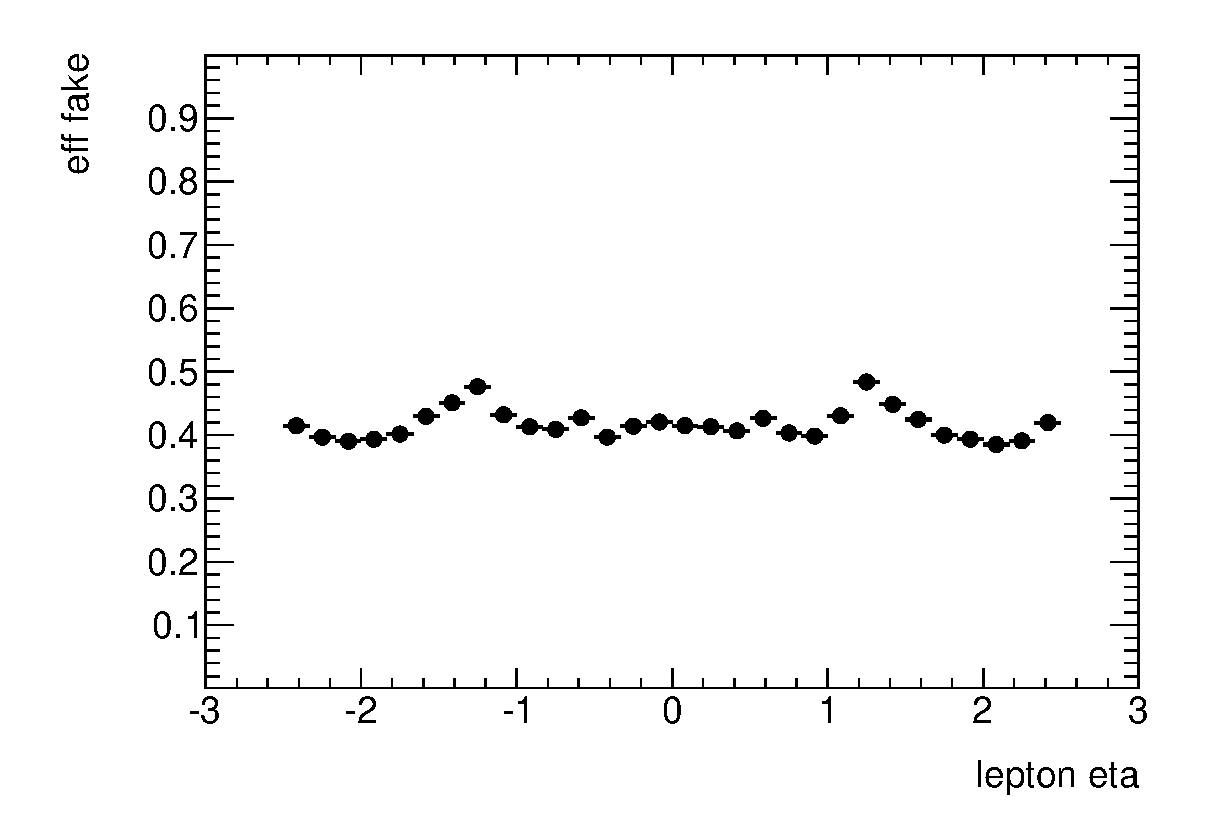
\includegraphics[width=.45\textwidth]{appendices/figures/mujets_mmB/fit_h_lep_eta_muon_fake_untagged}
\caption{Lepton $\eta$ dependency of $\epsilon_\mathrm{real}$ (left plot) and $\epsilon_\mathrm{fake}$ (right plot).}\label{fig:etaDep}
\end{figure} \begin{figure}\centering
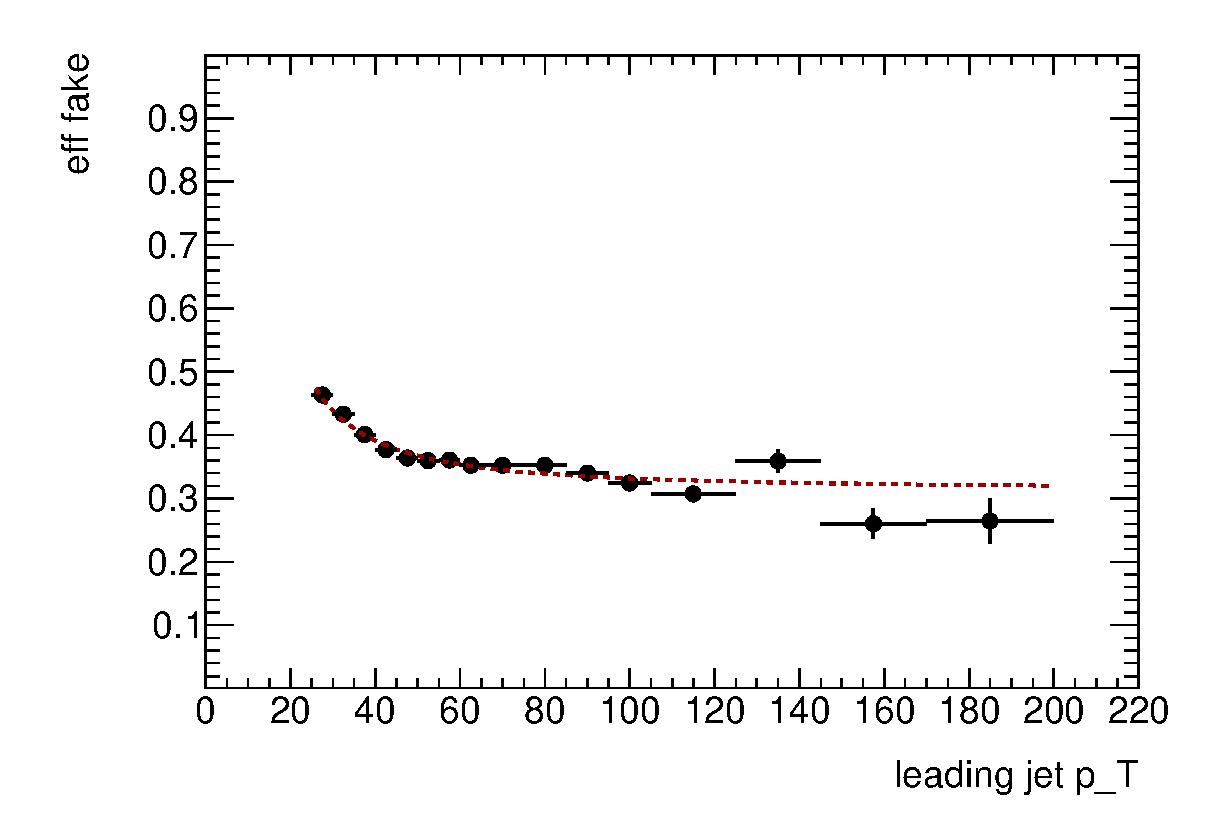
\includegraphics[width=.45\textwidth]{appendices/figures/mujets_mmB/fit_h_lep_LJpT_rb_muon_fake_untagged}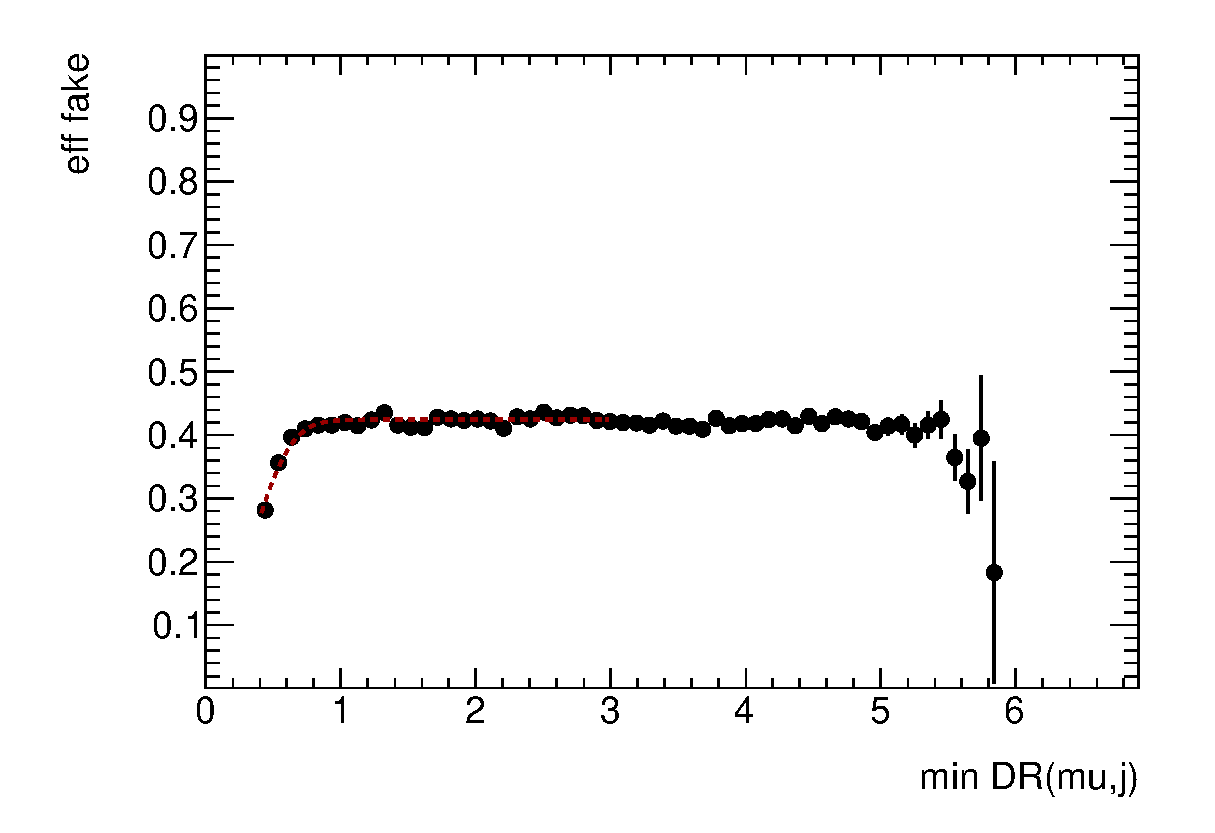
\includegraphics[width=.45\textwidth]{appendices/figures/mujets_mmB/fit_h_lep_minDR_muon_fake_untagged}
\caption{Parametrization of $\epsilon_\mathrm{fake}$ as a function of the leading jet $p_T$ (left plot) and of the minimum $\Delta R$ between muon and jets (right plot). }\label{fig:ljptmindrDep}
\end{figure} 

\begin{table}\centering
\begin{tabular}{l c c }
\toprule
 & $\epsilon_\mathrm{fake}$ &  $\epsilon_\mathrm{real}$  \\\midrule
untagged & $0.4178 \pm 0.0006 $ & $ 0.9805 \pm 0.0003 $ \\
tagged   & $0.353  \pm 0.002 $ & $ 0.973 \pm 0.006 $ \\\bottomrule
\end{tabular}\caption{Average values for $\epsilon_\mathrm{fake}$ and  $\epsilon_\mathrm{real}$ in untagged and tagged channels. Error is only statistical.}\label{tab:averageeffs}
\end{table} 

The two $\epsilon_\mathrm{fake}$ dependencies on  
leading jet $p_T$ and minimum $\Delta R$ between muon and 
jets  are then combined together to obtain a weight for the value of 
the fake efficiency at a given $\eta$:
\begin{equation}
\epsilon_\mathrm{fake} = \epsilon_\mathrm{fake}(\eta) \dfrac{f_{min\Delta R}(min\Delta R)}{<\epsilon_\mathrm{fake}^{min\Delta R}>}\dfrac{f_{LJpT}(LJpT)}{<\epsilon_\mathrm{fake}^{LJpT}>}.
\end{equation}

Figure~\ref{fig:datamc1} shows the agreement between data and Monte Carlo 
backgrounds 
when the QCD multi-jet backgorund estimated with this Matrix Method 
is considered. Here the events satisfy the full standard 
selection for top analyses~\cite{topCommonObjects2012} with 
exactly 1 jet before and after applying the triangular cut 
$E_T^{Miss} + m_T(W)>60~$GeV, which suppresses QCD multi-jet
contributions, and no \btag ging information is 
required. Adding the tagging selection leads to the comparison 
plots of Figure~\ref{fig:datamc2} where the full selection (with 
and without the triangular cut) leave exactly 2 jets of which at 
least one has been tagged as a \bjet. The variables $p_T(\mu)$, 
$E_T^{Miss}$ and $m_T(W)$ are chosen to illustrate the QCD multi-jet 
background prediction since it is known that here the QCD multi-jet will peak at 
low values. 
%In the Appendix~\ref{app:extradatamc} more plots 
%for other jet multiplicities can be found.



\begin{figure}[htb]\centering
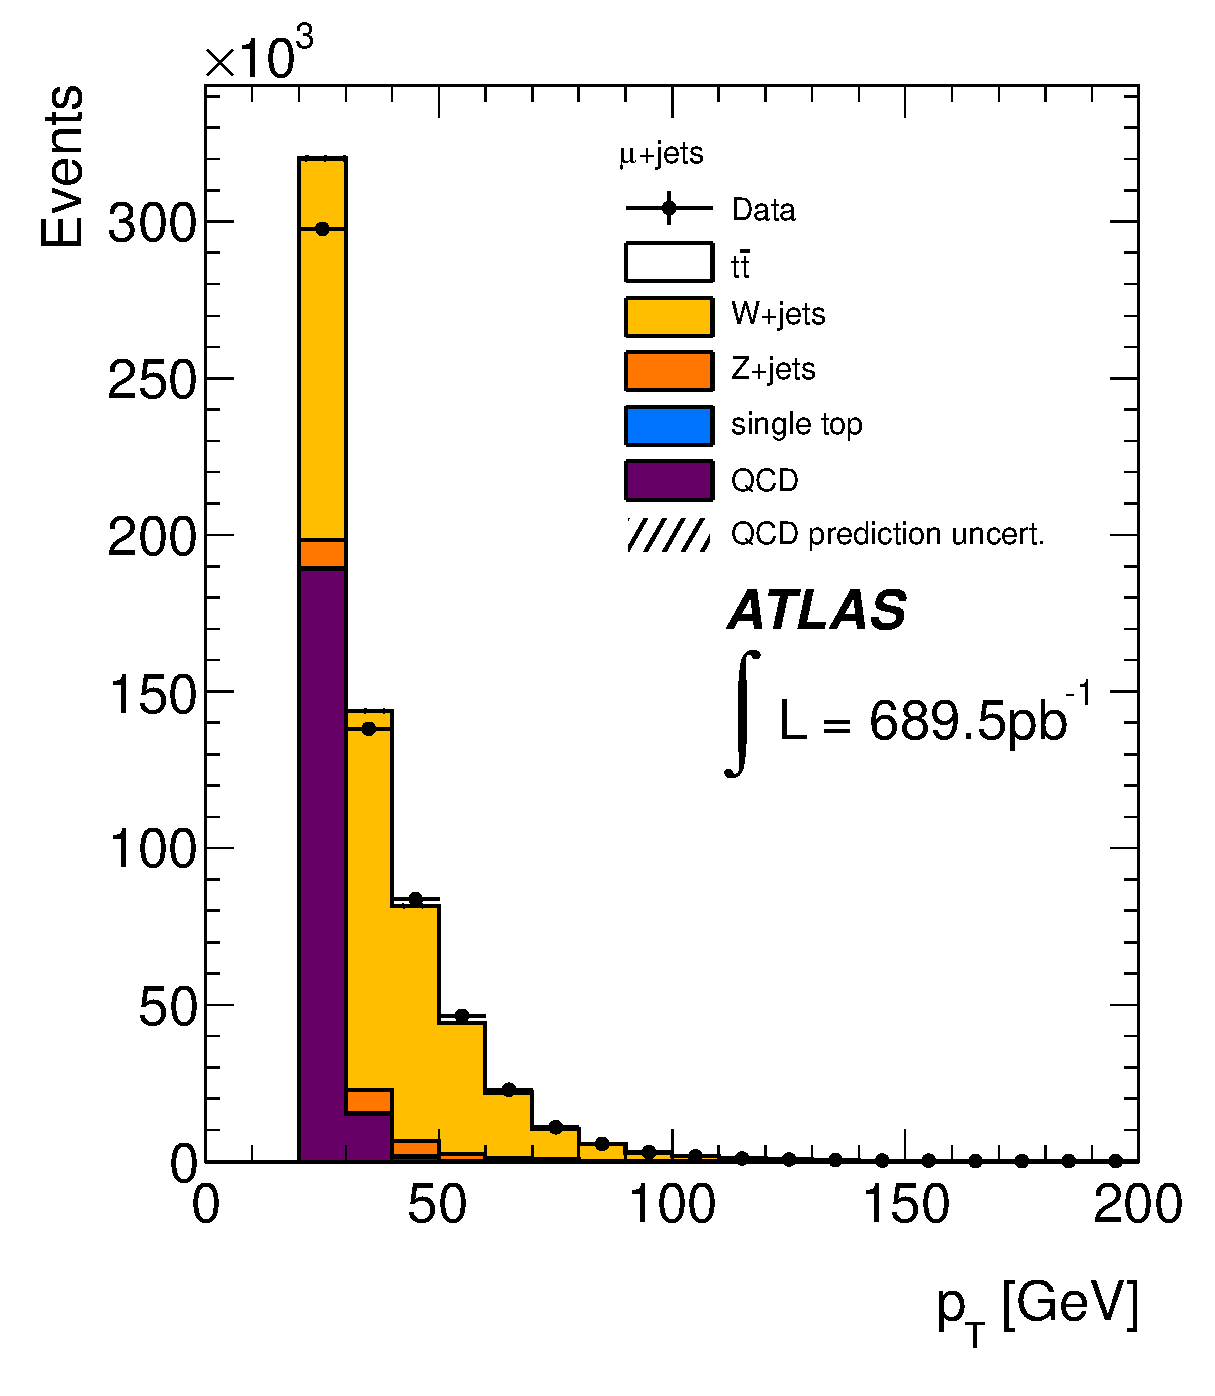
\includegraphics[width=.3\textwidth]{{appendices/figures/mujets_mmB/hpresel_muon_pT_0btagin5.85SV0_1jetex25_MUON_MET20_HTAll0}.eps}
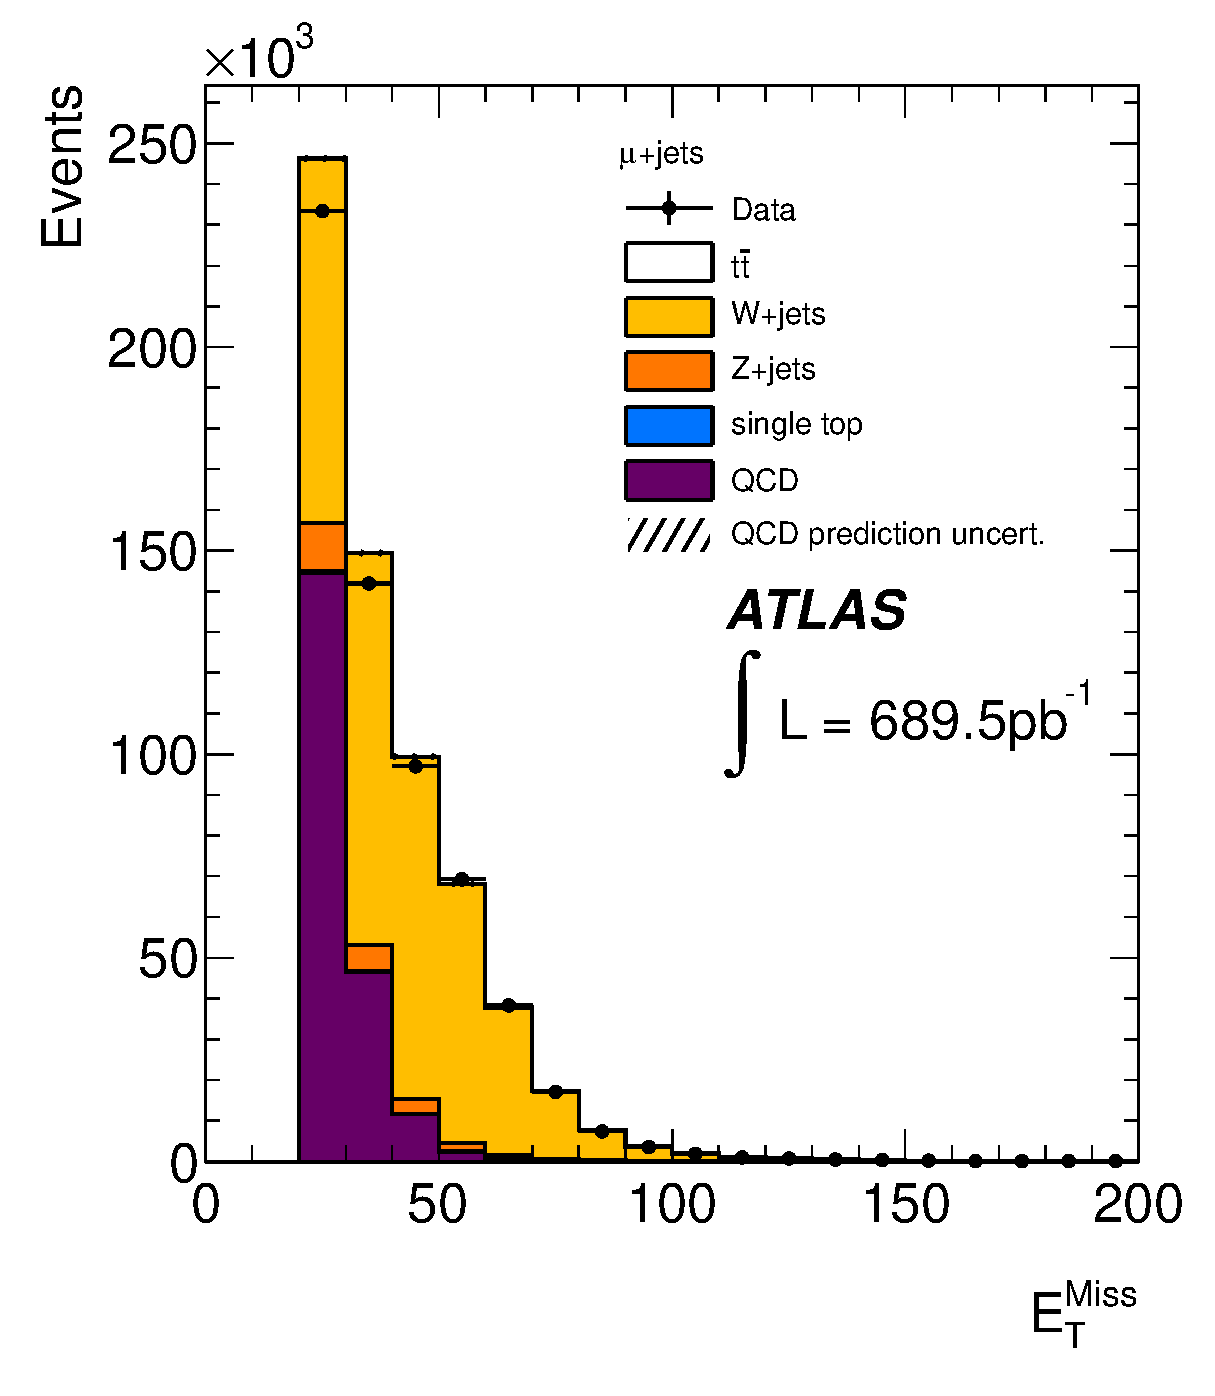
\includegraphics[width=.3\textwidth]{{appendices/figures/mujets_mmB/hpresel_missingET_missET_0btagin5.85SV0_1jetex25_MUON_MET20_HTAll0}.eps}
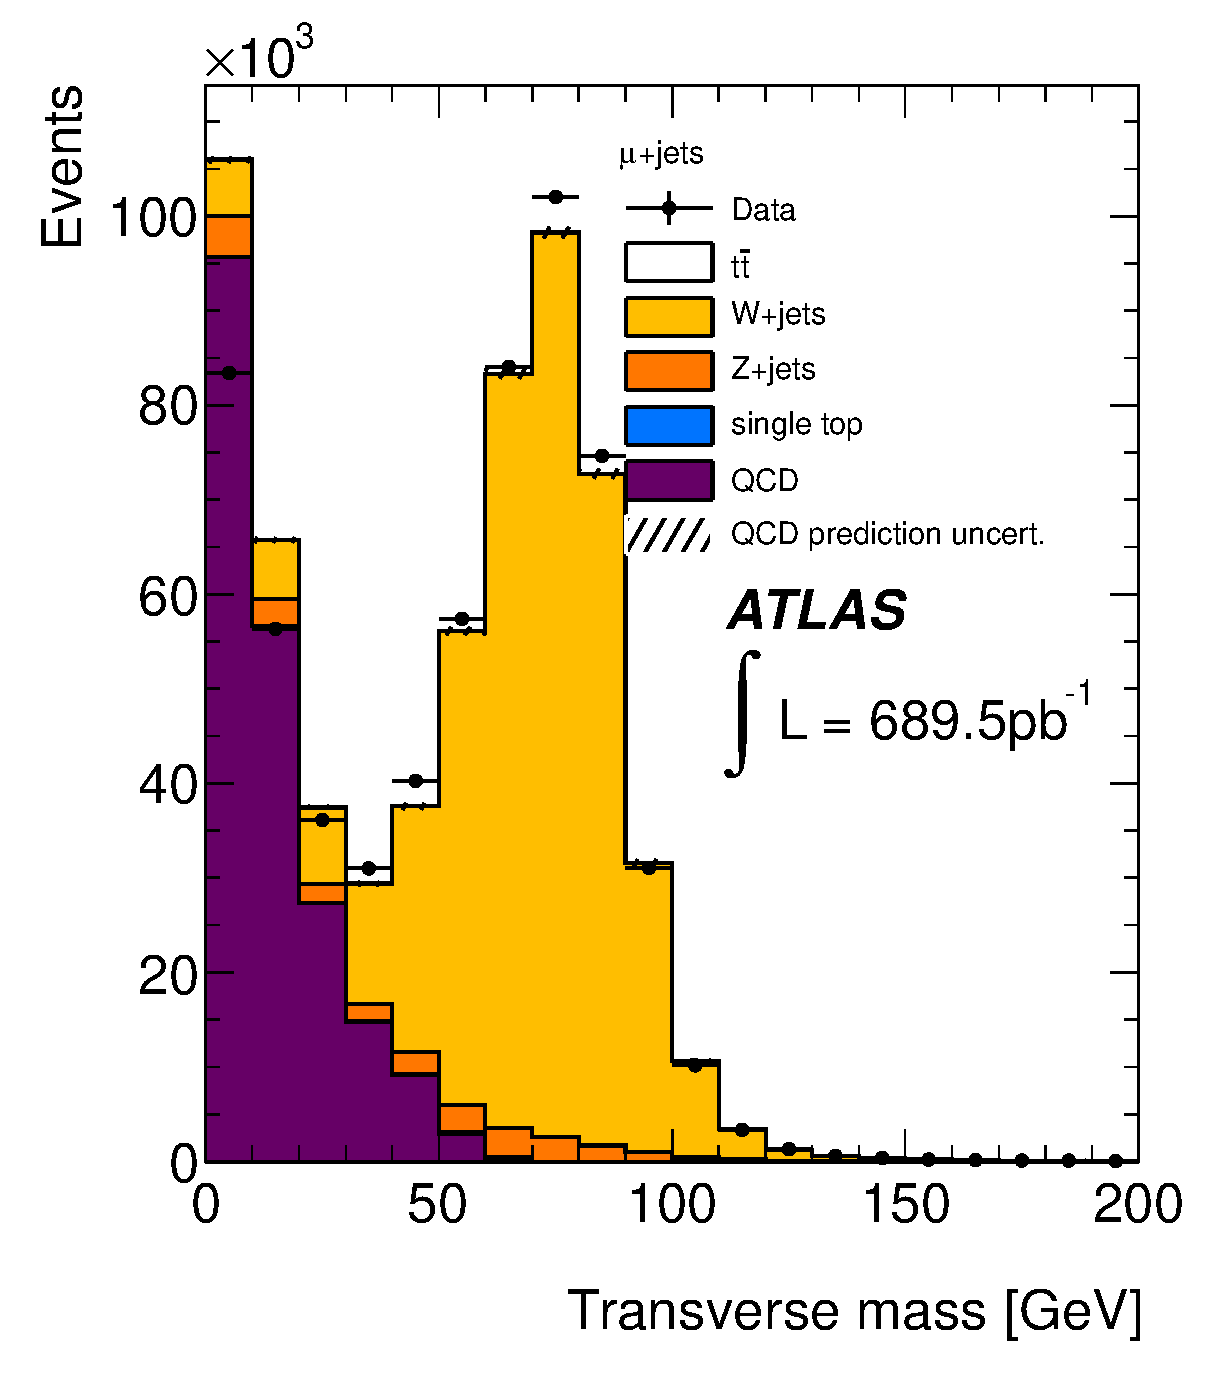
\includegraphics[width=.3\textwidth]{{appendices/figures/mujets_mmB/hmuon_Wlep_MassT_0btagin5.85SV0_1jetex25_MUON_MET20_HTAll0}.eps}\\
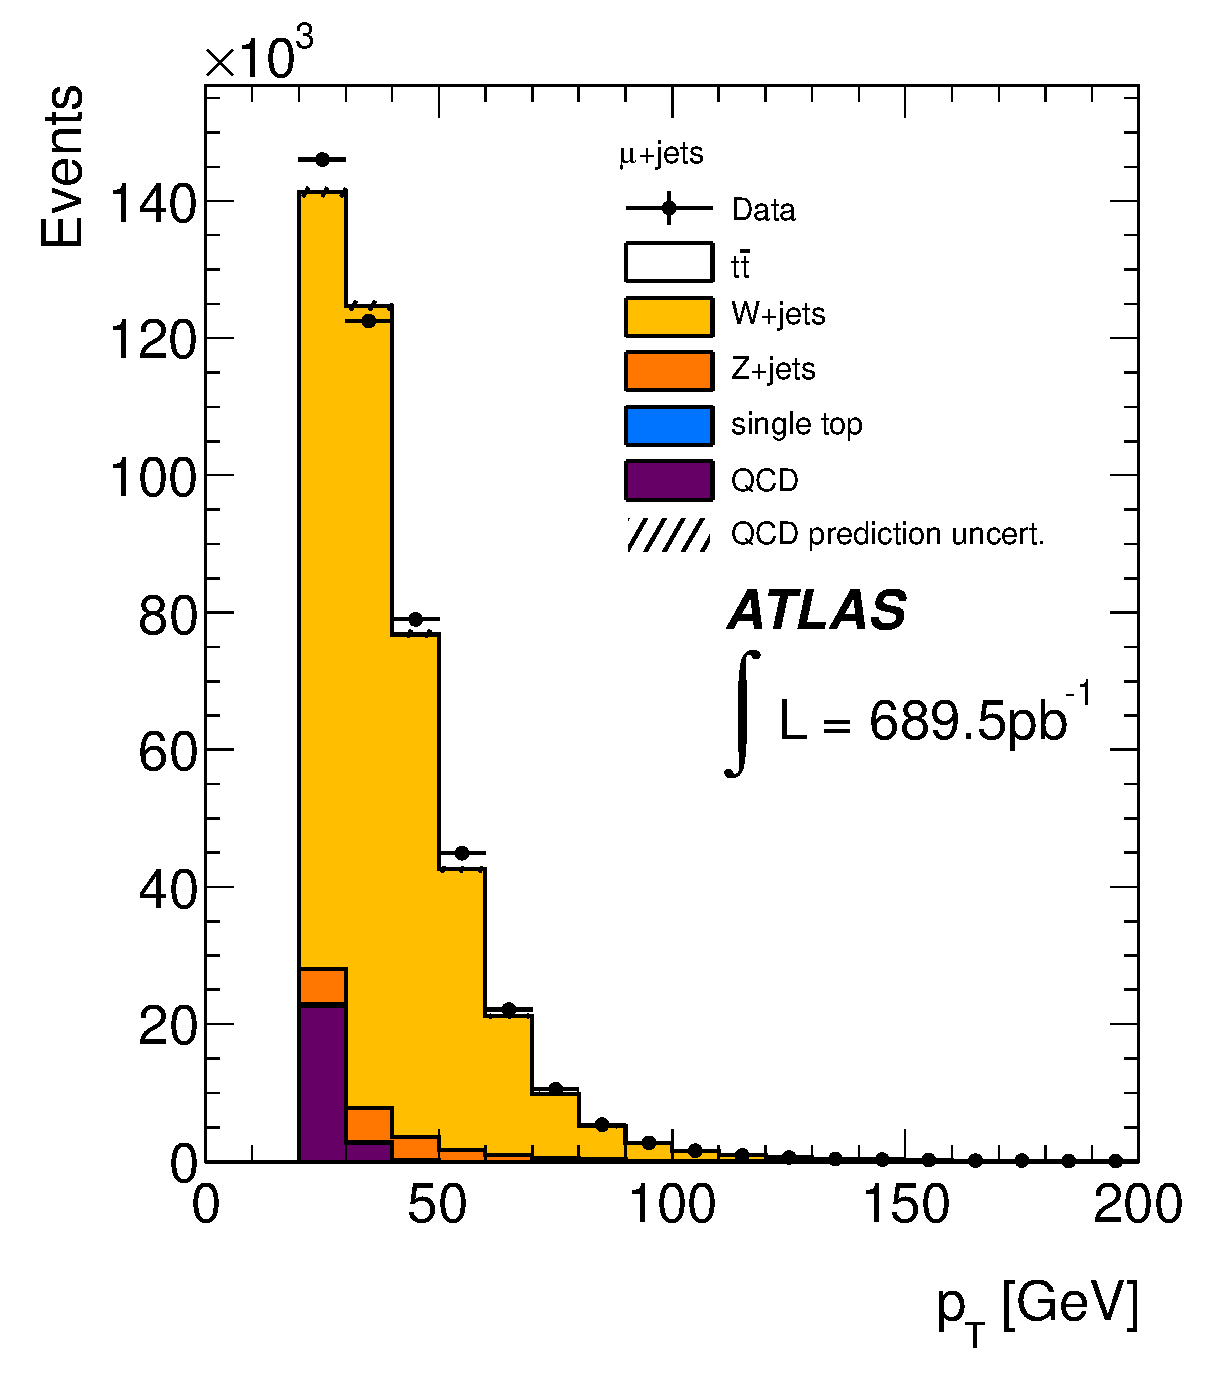
\includegraphics[width=.3\textwidth]{{appendices/figures/mujets_mmB/hpresel_muon_pT_0btagin5.85SV0_1jetex25_MUON_MET20_MTW_MET60_-1}.eps}
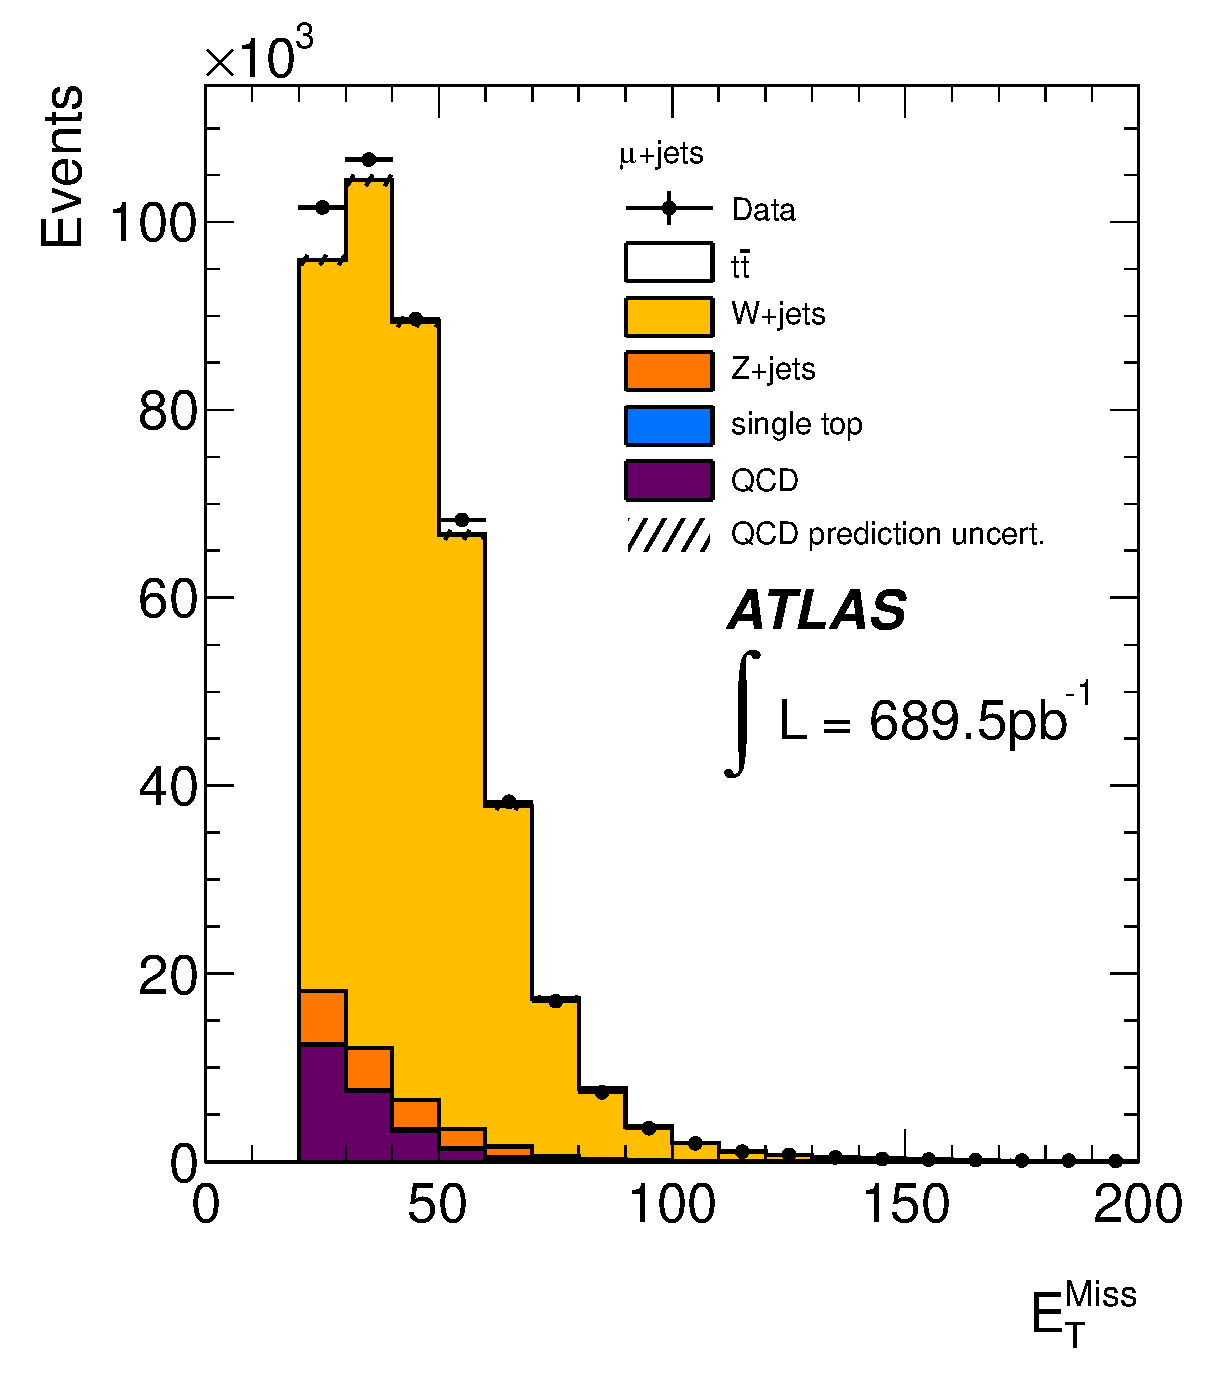
\includegraphics[width=.3\textwidth]{{appendices/figures/mujets_mmB/hpresel_missingET_missET_0btagin5.85SV0_1jetex25_MUON_MET20_MTW_MET60_-1}.eps}
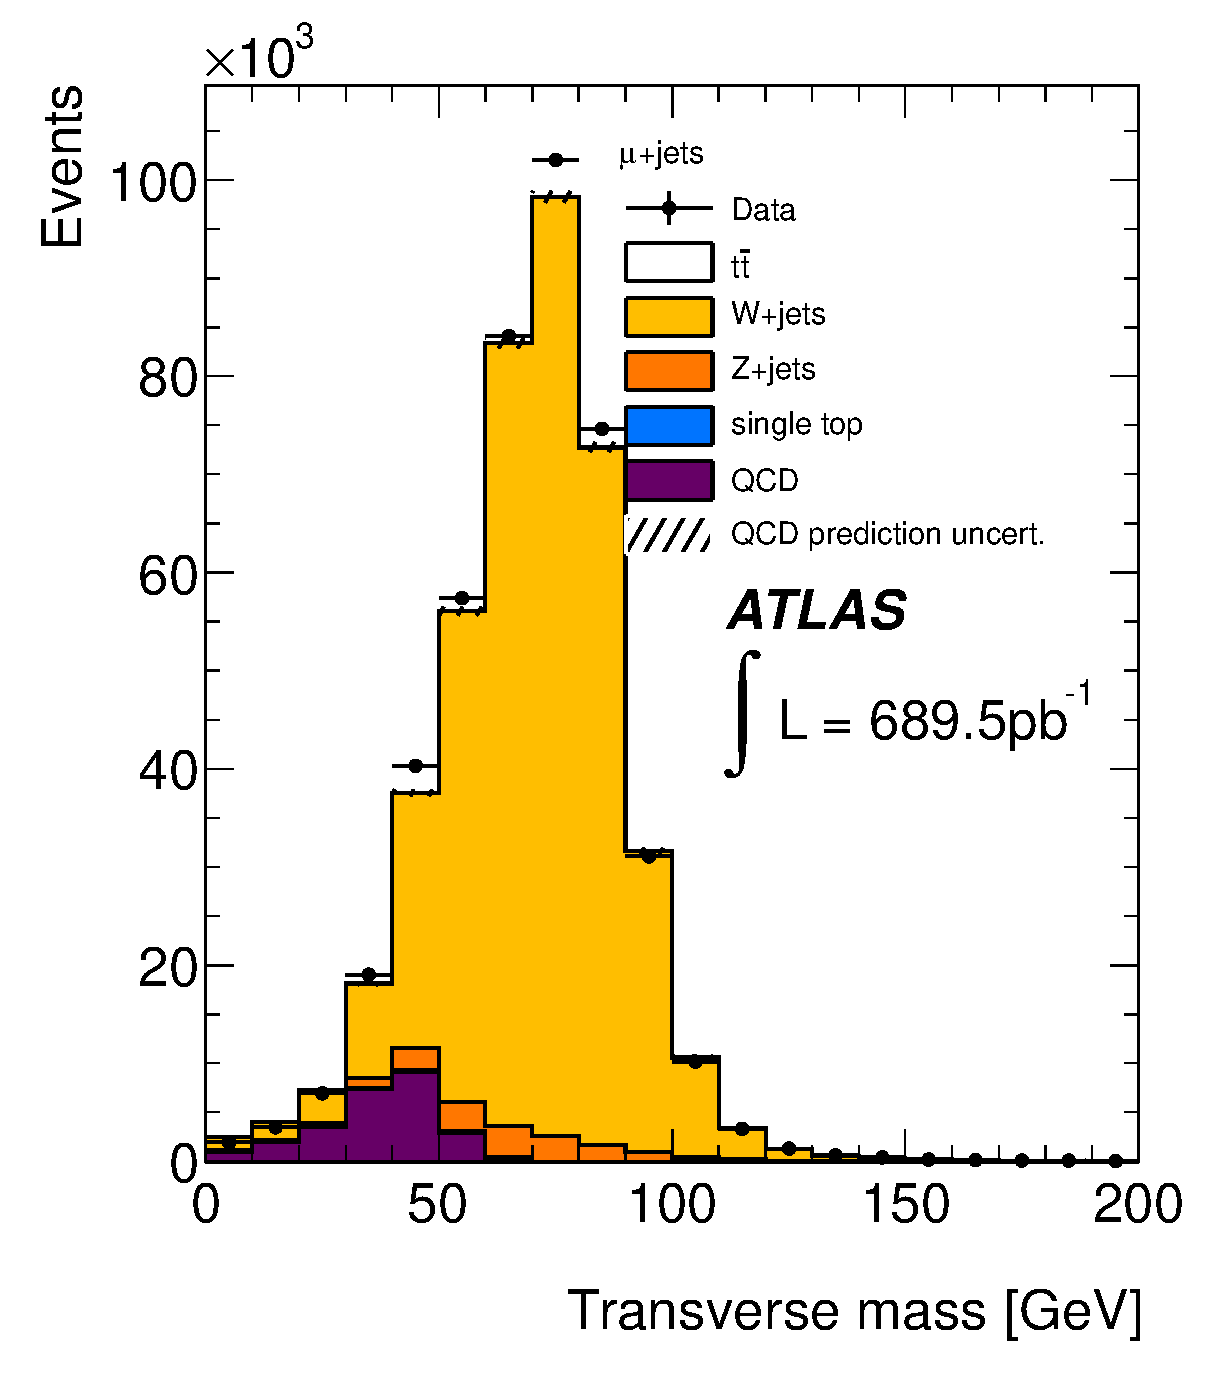
\includegraphics[width=.3\textwidth]{{appendices/figures/mujets_mmB/hmuon_Wlep_MassT_0btagin5.85SV0_1jetex25_MUON_MET20_MTW_MET60_-1}.eps}
\caption{Comparison plots between data and backgrounds for the muon transverse momentum (left column), missing transverse energy (central column) and the transverse mass of the $W$ (right column). The full event selection of 1 jet exclusive with no btagging information is used without and with the triangular cut (top and bottom respectively).}\label{fig:datamc1}
\end{figure} 
\begin{figure}[htb]\centering
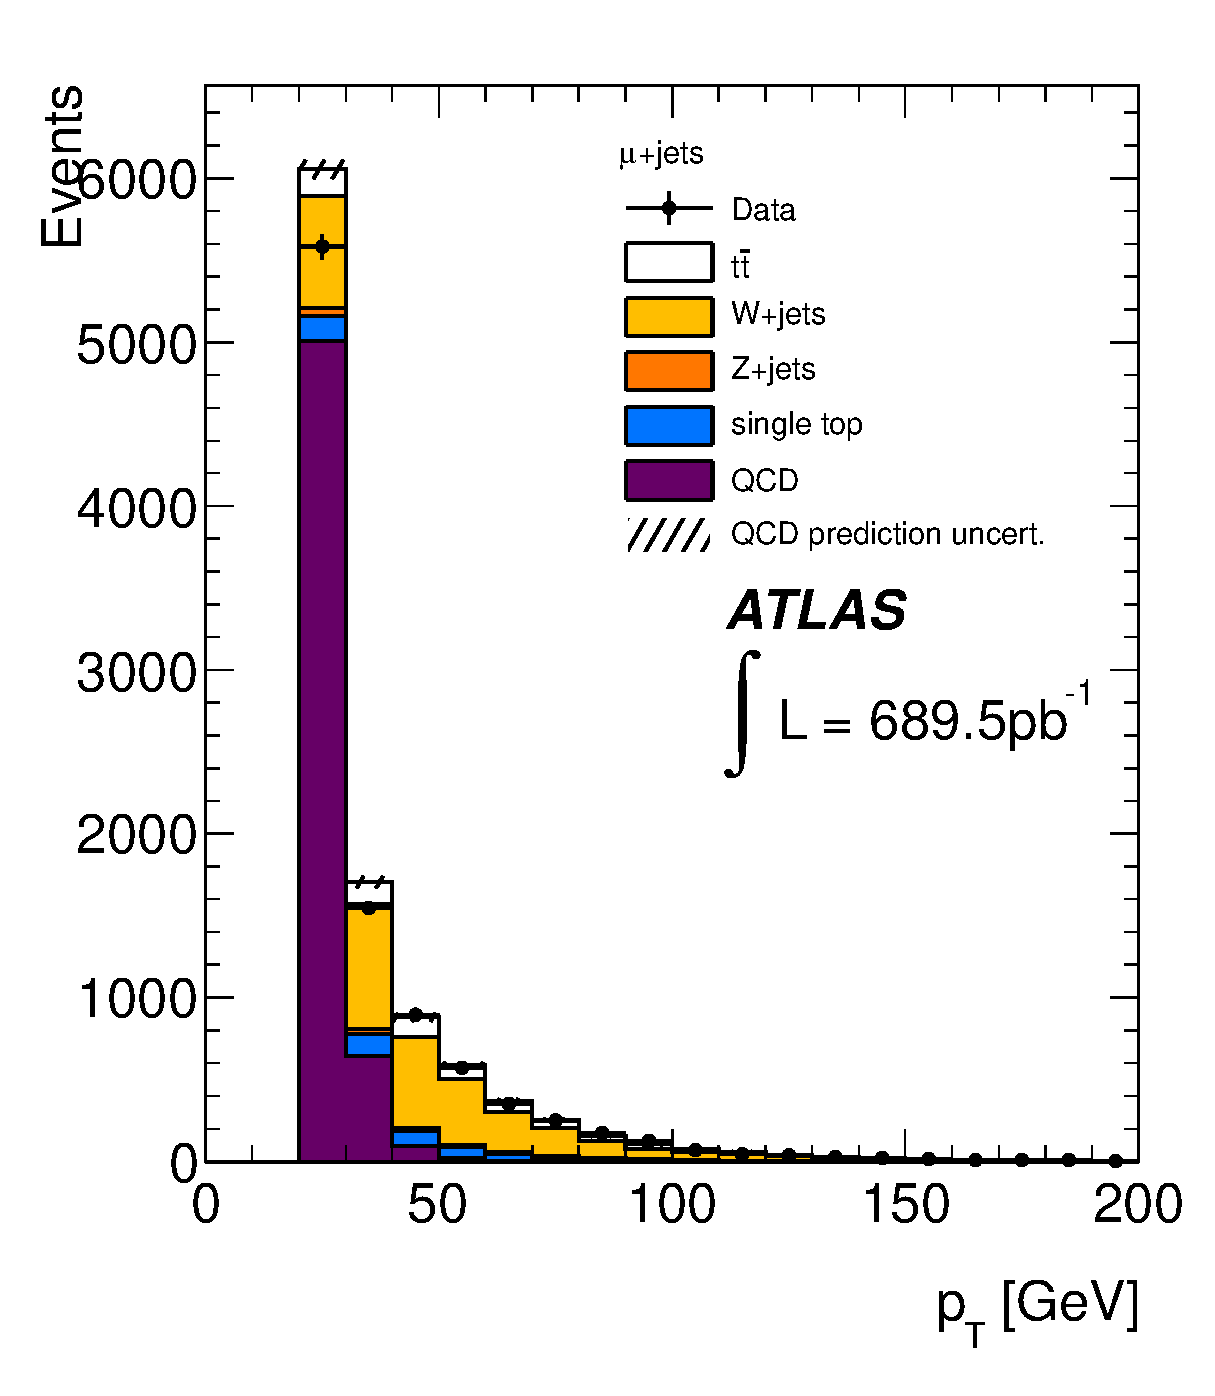
\includegraphics[width=.3\textwidth]{{appendices/figures/mujets_mmB/hpresel_muon_pT_1btagin5.85SV0_2jetex2525_MUON_MET20_HTAll0}.eps}
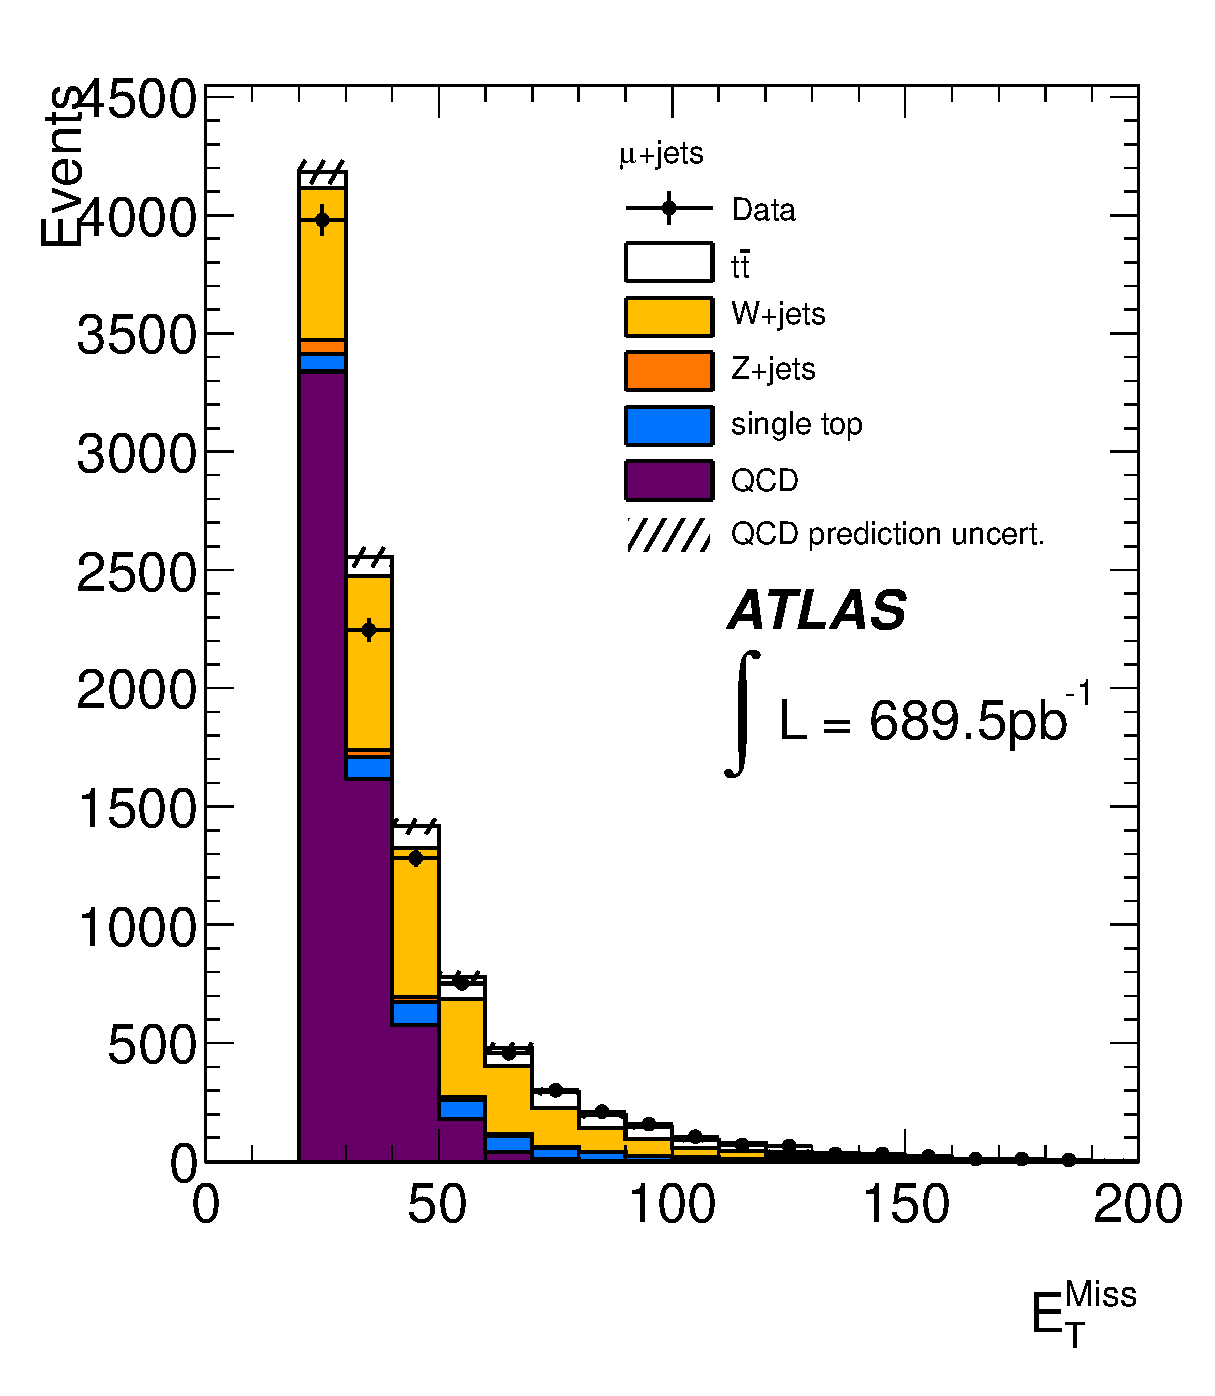
\includegraphics[width=.3\textwidth]{{appendices/figures/mujets_mmB/hpresel_missingET_missET_1btagin5.85SV0_2jetex2525_MUON_MET20_HTAll0}.eps}
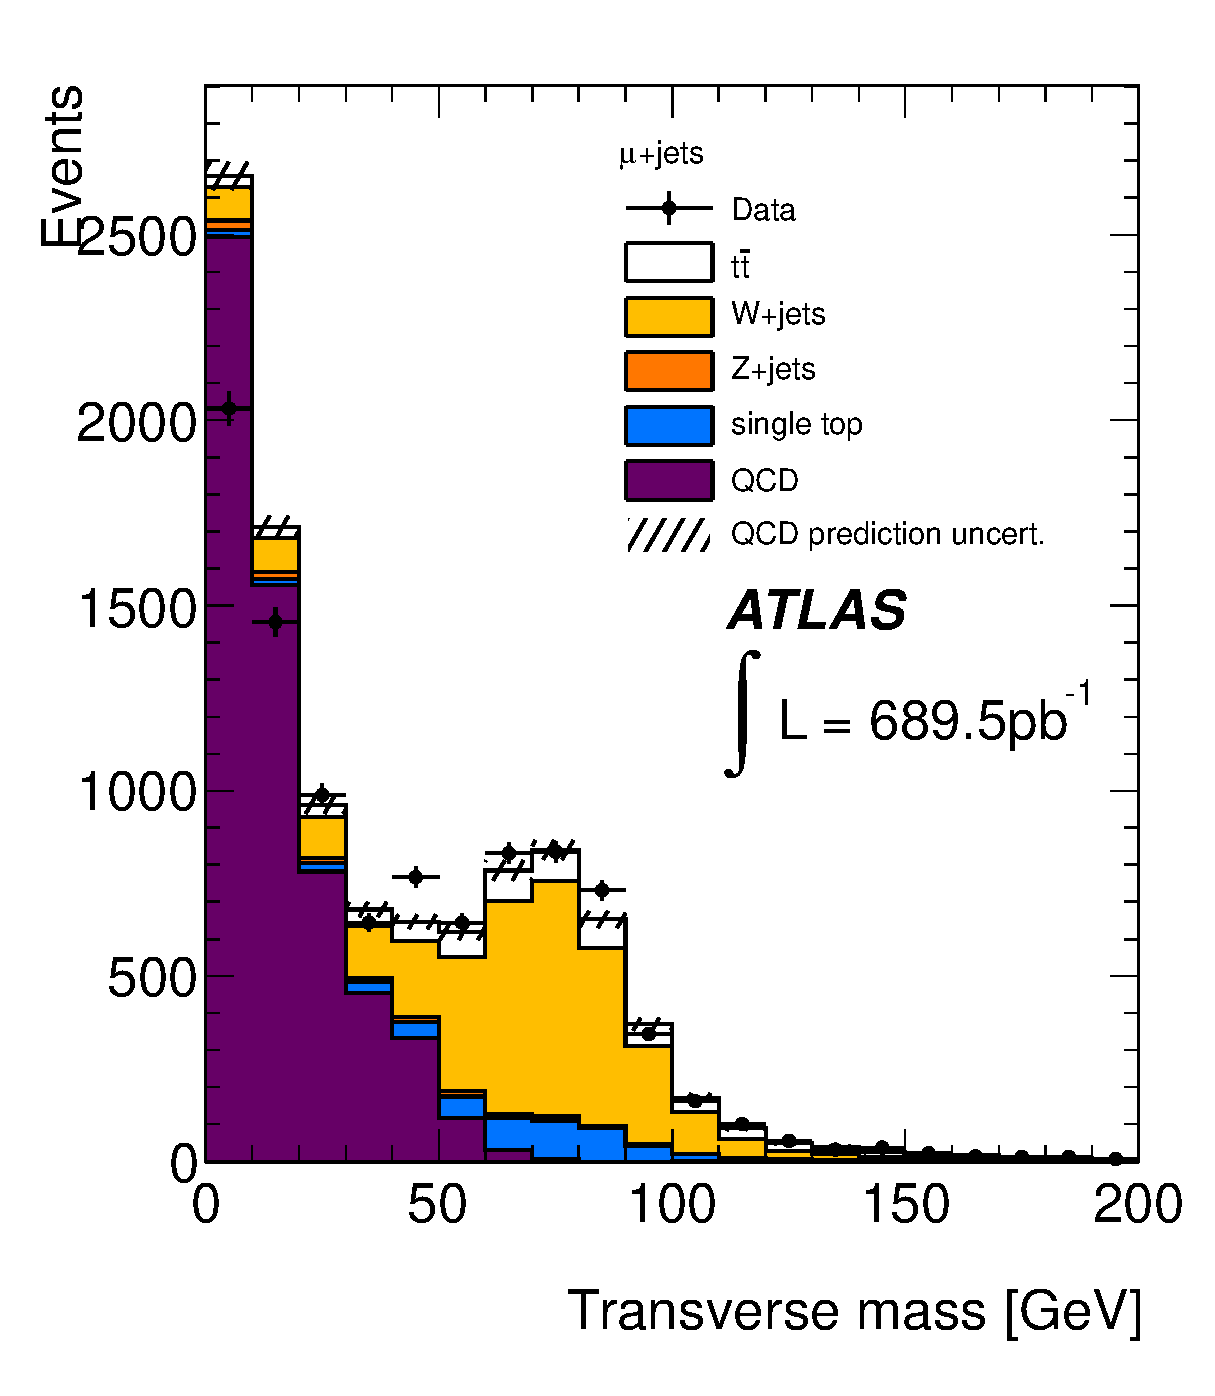
\includegraphics[width=.3\textwidth]{{appendices/figures/mujets_mmB/hmuon_Wlep_MassT_1btagin5.85SV0_2jetex2525_MUON_MET20_HTAll0}.eps}\\
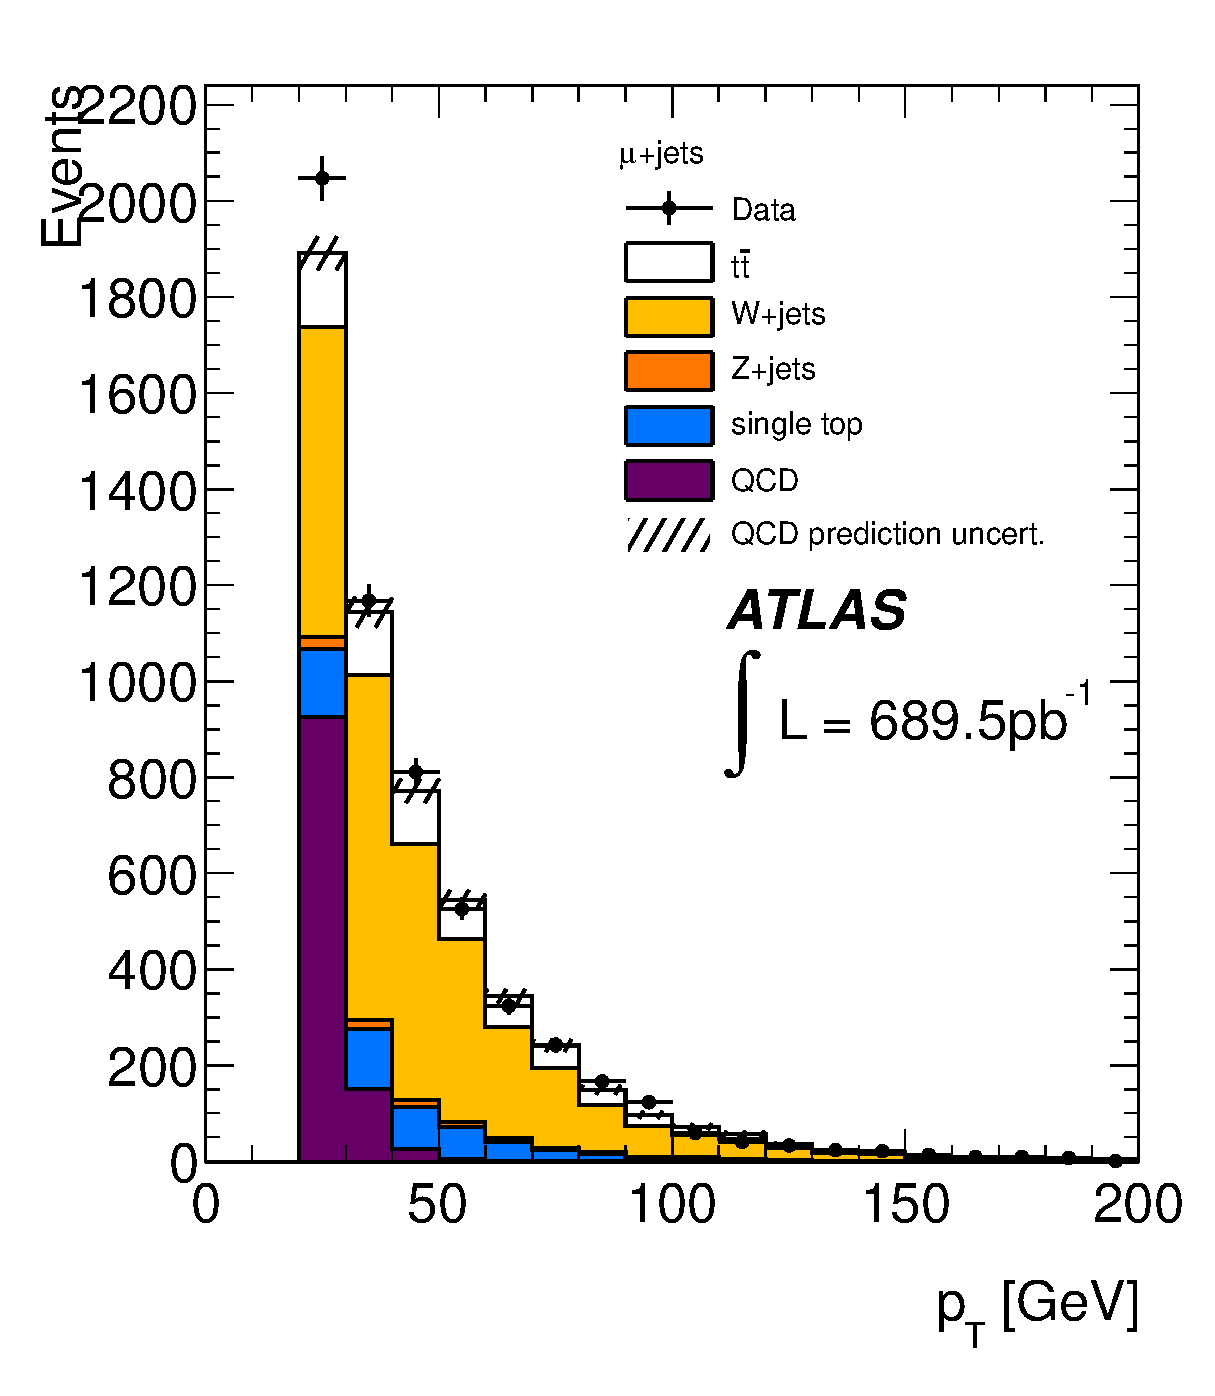
\includegraphics[width=.3\textwidth]{{appendices/figures/mujets_mmB/hpresel_muon_pT_1btagin5.85SV0_2jetex2525_MUON_MET20_MTW_MET60_-1}.eps}
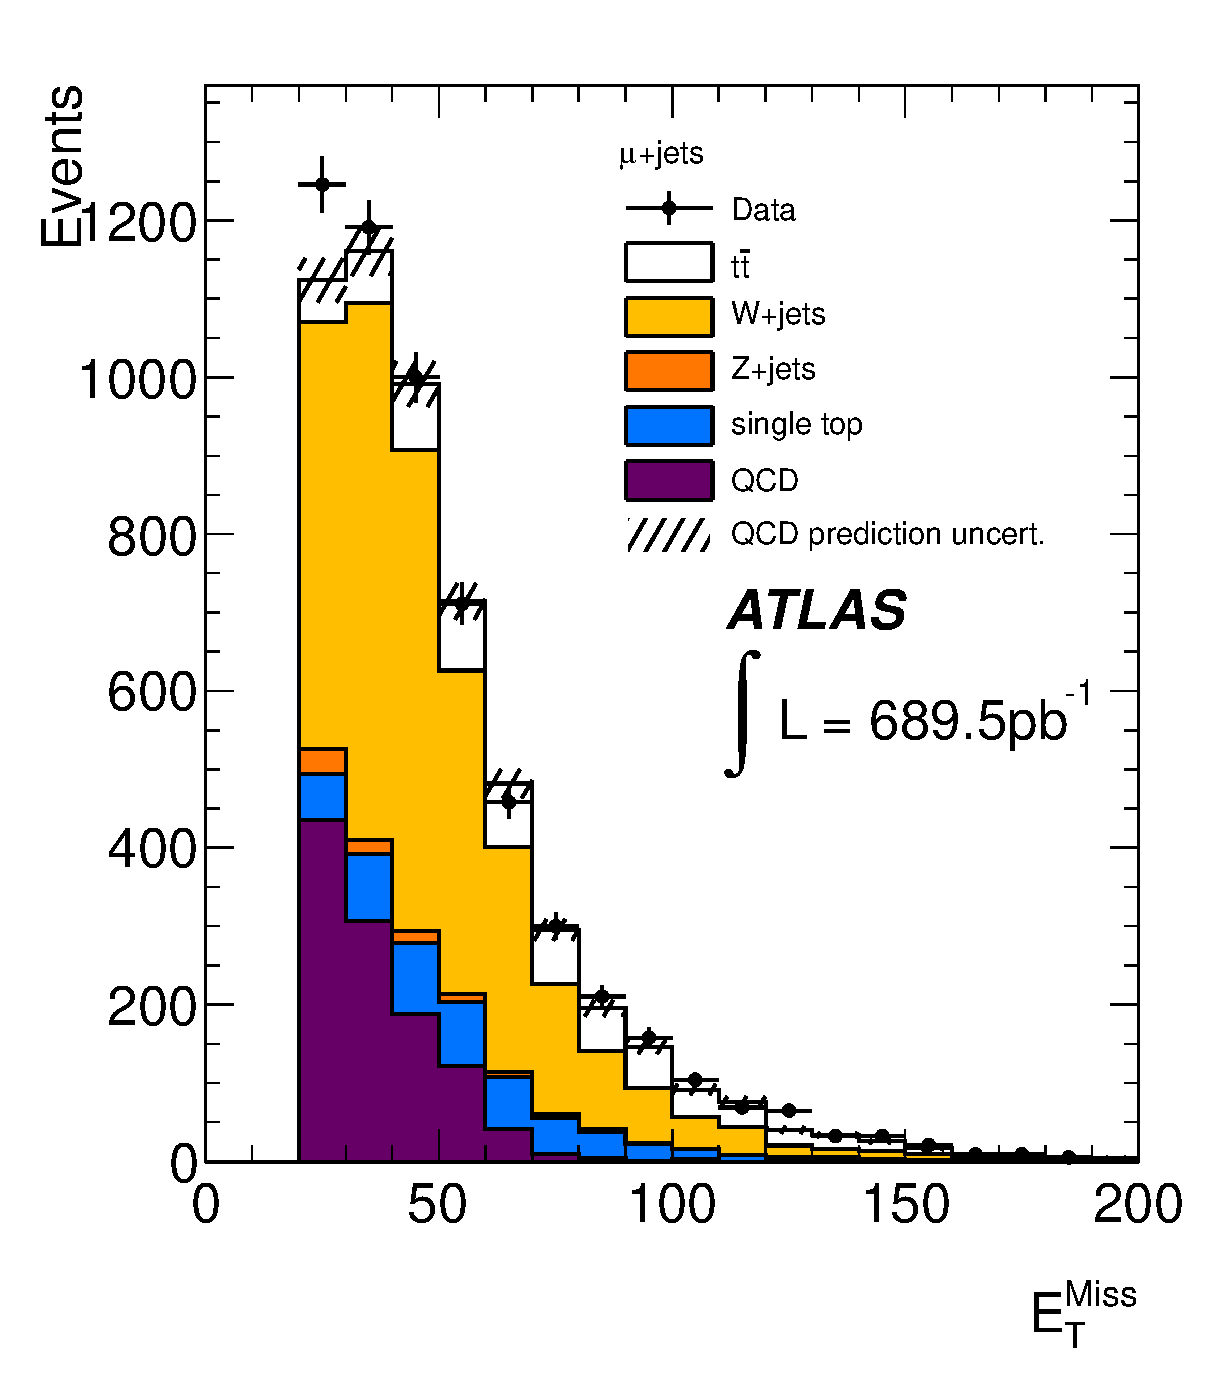
\includegraphics[width=.3\textwidth]{{appendices/figures/mujets_mmB/hpresel_missingET_missET_1btagin5.85SV0_2jetex2525_MUON_MET20_MTW_MET60_-1}.eps}
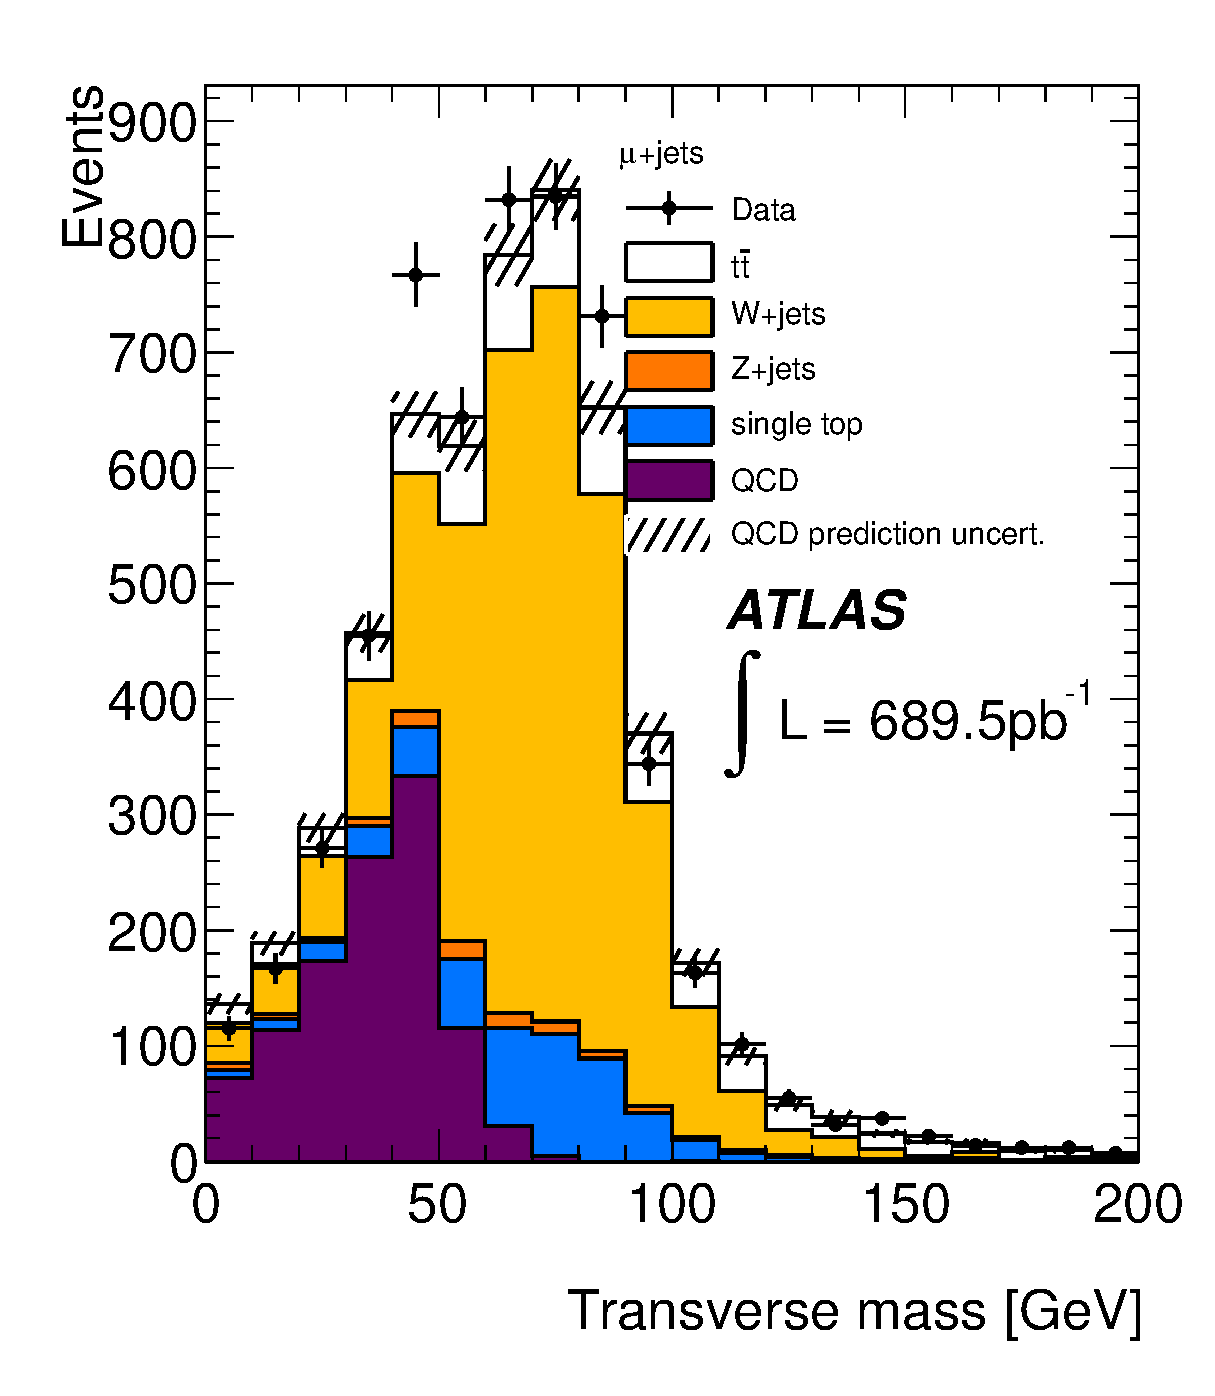
\includegraphics[width=.3\textwidth]{{appendices/figures/mujets_mmB/hmuon_Wlep_MassT_1btagin5.85SV0_2jetex2525_MUON_MET20_MTW_MET60_-1}.eps}
\caption{Comparison plots between data and backgrounds for the muon transverse momentum (left column), missing transverse energy (central column) and the transverse mass of the $W$ (right column). The full event selection of 2 jet exclusive with at least 1 btagged jet is used without and with the triangular cut (top and bottom respectively).}\label{fig:datamc2}
\end{figure} 


The two plots in Figure~\ref{fig:jetmultiplicity} show the 
total amount of events for data and backgrounds in the pre-tagged 
and \btag ged channels in different jet multiplicity bins. 
The numerical values for the QCD estimate are reported in 
Table~\ref{tab:yieldsuntagged} and Table~\ref{tab:yieldstagged} 
for the pre-tagged and \btag ged case respectively.

\begin{figure}[htb]\centering
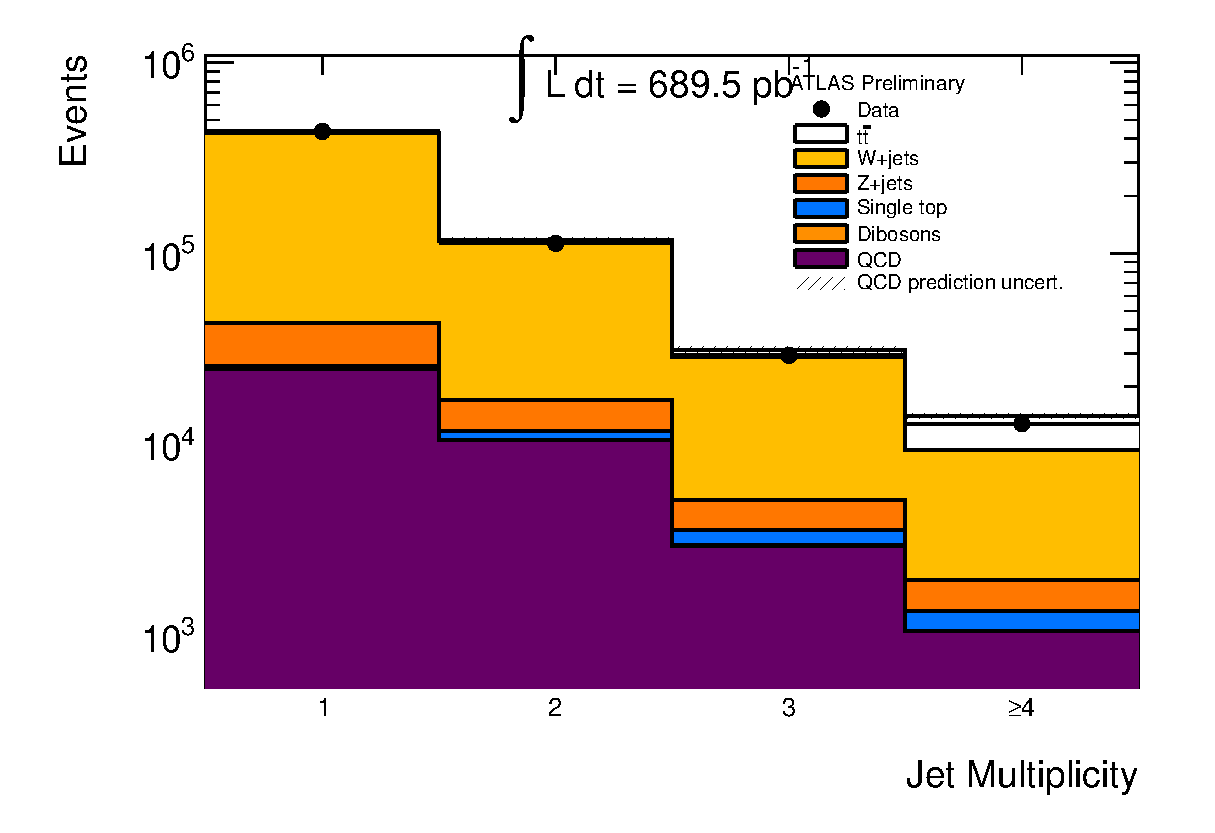
\includegraphics[width=.45\textwidth]{{appendices/figures/mujets_mmB/nJets_MUON_0btagin5.85SV0_MET20_MTW_MET60_-1}.eps}
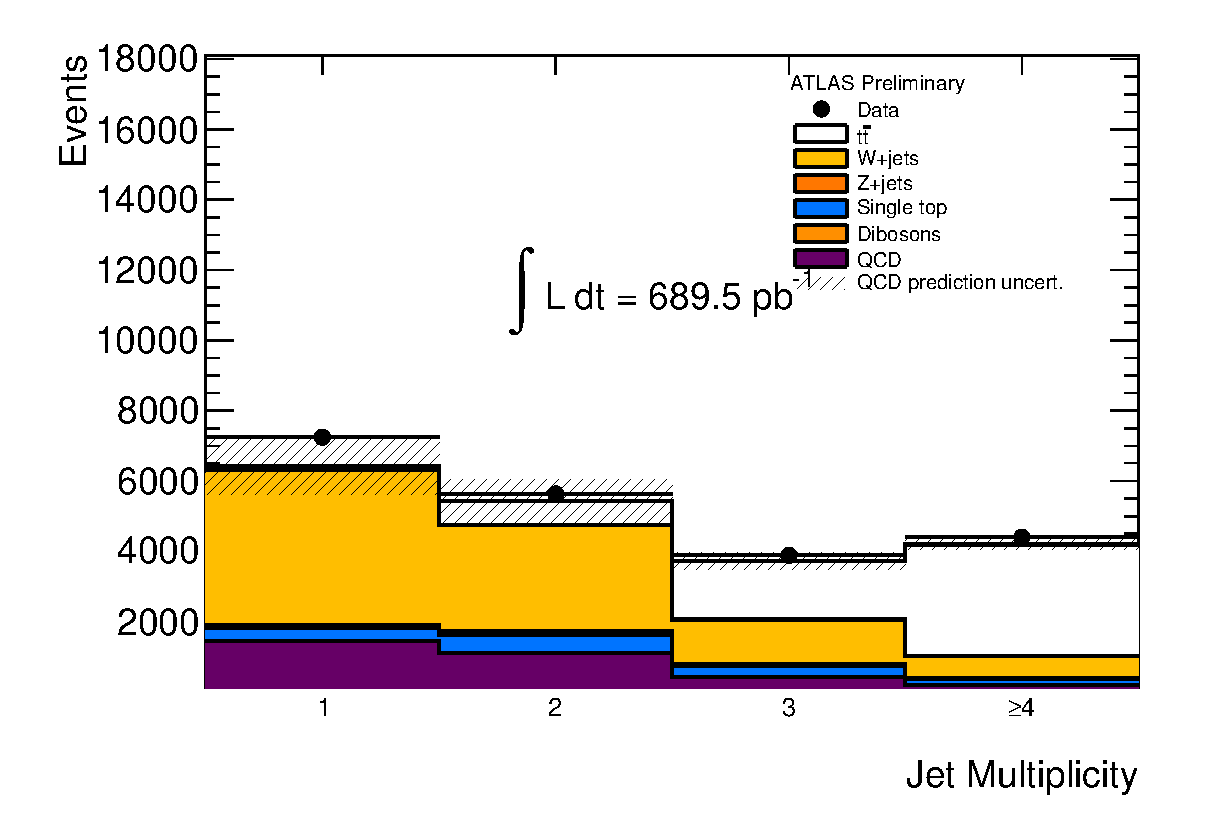
\includegraphics[width=.45\textwidth]{{appendices/figures/mujets_mmB/nJets_MUON_1btagin5.85SV0_MET20_MTW_MET60_-1}.eps}
\caption{Yields plots for data and backgrounds requiring full event selection (left plot) and full event selection plus at least one btagged jet (right plot) in jet multiplicity bins.}\label{fig:jetmultiplicity}
\end{figure}

\begin{table}[h!tb]\centering
\resizebox{1.\textwidth}{!}{
\begin{tabular}{l c c c c}
\toprule
 & = 1 jet & = 2 jets & = 3 jets & $\ge$ 4 jets \\
\midrule
$t\bar{t}$& 304.33 $\pm$  7.41 &1320.55 $\pm$  15.50 &2709.63 $\pm$  22.13 &4702.33 $\pm$29.49\\
QCD & 24803.36 $\pm$  153.57 &10511.66 $\pm$  87.94 &2942.08 $\pm$  43.72 &1049.85 $\pm$25.02\\
W+jets& 385242.06 $\pm$  1129.55 &98826.98 $\pm$  373.93 &23614.51 $\pm$  154.62 &7419.73 $\pm$81.07\\
Z+jets& 17257.90 $\pm$  63.81 &5478.57 $\pm$  35.64 &1553.30 $\pm$  18.79 &592.78 $\pm$11.28\\
Single top& 1002.70 $\pm$  10.77 &1126.85 $\pm$  10.55 &578.51 $\pm$  6.47 &285.44 $\pm$4.15\\
\midrule
Total prediction & 428610.34 $\pm$1141.80 & 117264.61 $\pm$386.23 & 31398.04 $\pm$163.41 & 14050.14 $\pm$90.62 \\
Data& 437526 &112984 &29135 &12779\\
\bottomrule
\end{tabular}}
\caption{Yields table for the data and background samples for different jet multiplicities in the untagged full event selection.}\label{tab:yieldsuntagged}
\end{table} 


\begin{table}[h!tb]\centering
\resizebox{1.\textwidth}{!}{
\begin{tabular}{l c c c c}
\toprule
 & = 1 jet & = 2 jets & = 3 jets & $\ge$ 4 jets \\
\midrule
$t\bar{t}$& 108.35 $\pm$  4.22 &689.18 $\pm$  10.58 &1659.28 $\pm$  16.48 &3185.88 $\pm$23.19\\
QCD & 1449.22 $\pm$  29.45 &1109.84 $\pm$  24.17 &420.08 $\pm$  14.44 &211.11 $\pm$10.35\\
W+jets& 4392.92 $\pm$  77.83 &3016.70 $\pm$  56.17 &1280.12 $\pm$  38.41 &612.50 $\pm$26.04\\
Z+jets& 104.68 $\pm$  4.76 &94.69 $\pm$  4.56 &52.10 $\pm$  3.32 &28.77 $\pm$2.44\\
Single top& 359.78 $\pm$  6.16 &522.23 $\pm$  6.80 &307.53 $\pm$  4.50 &159.42 $\pm$2.96\\
\midrule
Total prediction & 6414.95 $\pm$83.69 & 5432.64 $\pm$62.60 & 3719.11 $\pm$44.57 & 4197.68 $\pm$36.58 \\
Data& 7243 &5634 &3876 &4406\\
\bottomrule
\end{tabular}}
\caption{Yields table for the data and background samples for different jet multiplicities in the tagged full event selection (at least one bjet).}\label{tab:yieldstagged}
\end{table} 


An estimation of the systematic uncertainties on the QCD multi-jet background
as derived in this Matrix Method
can be evaluated considering the following sources:
\begin{enumerate}
 \item statistical error on  $\epsilon_\mathrm{fake}$ and  $\epsilon_\mathrm{real}$;
\item statistical error on the QCD estimation;
\item different control regions for the estimation of fake efficiency;
\item changes in the parametrization used.
\end{enumerate} 
For the points 1 and 2, the values can be taken from what already 
shown in Table~\ref{tab:averageeffs} and 
Tables~\ref{tab:yieldsuntagged}~and~\ref{tab:yieldstagged}. For what 
concerns point 3, we compared the results obtained in control region 
$5$~GeV$< E^{Miss}_T<15$~GeV with an estimation in control region 
$ E^{Miss}_T<10$~GeV, while no studies have yet been performed about 
point 4. Table~\ref{tab:systuncertuntag}~and~\ref{tab:systuncerttag} 
summarize the systematic uncertainties for different jet multiplicity 
in the untagged and tagged channels respectively.


\begin{table}[h!tb]\centering
\begin{tabular}{l c c c c}
\toprule
 & = 1 jet & = 2 jets & = 3 jets & $\ge$ 4 jets \\
\midrule
$\varepsilon_1 $ & \multicolumn{4}{c}{ 0.1\% } \\
%QCD & 24803.36 $\pm$  153.57 &10511.66 $\pm$  87.94 &2942.08 $\pm$  43.72 &1049.85 $\pm$25.02\\
$\varepsilon_2 $ &  0.6\% & 0.8\% & 1.5\% & 2.4\% \\
%$\varepsilon_3 $ &  \\
$\varepsilon_3 $ & 7.9\% &  21.2\% &   31.0\% &   41.3\% \\\bottomrule
\end{tabular}\caption{Systematic uncertainties on QCD estimation for different jet multiplicity in the untagged case.}\label{tab:systuncertuntag}
%\end{table} 
%\begin{table}[hbt]\centering
\begin{tabular}{l c c c c}
\toprule
 & = 1 jet & = 2 jets & = 3 jets & $\ge$ 4 jets \\
\midrule
$\varepsilon_1 $ & \multicolumn{4}{c}{ 0.5\% } \\
%QCD & 1449.22 $\pm$  29.45 &1109.84 $\pm$  24.17 &420.08 $\pm$  14.44 &211.11 $\pm$10.35\\
$\varepsilon_2 $ &  2.0\% & 2.2\% & 3.4\% & 4.9\% \\
%$\varepsilon_3 $ &  \\
$\varepsilon_3 $ & 6.4\% &  18.5\% &   26.5\% &   32.4\% \\\bottomrule
\end{tabular}\caption{Systematic uncertainties on QCD estimation for different jet multiplicity in the tagged case.}\label{tab:systuncerttag}
\end{table} 




%\begin{figure}[htb]\begin{center}
%	\subfigure[]{\label{fig:MMmindr}
%        \begin{overpic}[width=0.47\textwidth]{vlq_analysis/figures/qcd_eff/fit_h_lep_minDR_muon_fake}
%        \put(0,50){\small \rotatebox{90}{$\varepsilon_{\rm fake}$}}
%        \put(70,0){\footnotesize min$\Delta R(\mu,j)$}
%        \end{overpic}
%        }
%  	%\includegraphics[width=0.47\textwidth]{vlq_analysis/figures/qcd_eff/fit_h_lep_minDR_muon_fake}}
%	\subfigure[]{\label{fig:MMmindr}
%        \begin{overpic}[width=0.47\textwidth]{vlq_analysis/figures/qcd_eff/fit_h_lep_LJpT_rb_muon_fake}
%        \put(0,50){\small \rotatebox{90}{$\varepsilon_{\rm fake}$}}
%        \put(60,0){\footnotesize leading jet $p_T$ [GeV]}
%        \end{overpic}
%        }
%  	%\includegraphics[width=0.47\textwidth]{vlq_analysis/figures/qcd_eff/fit_h_lep_LJpT_rb_muon_fake}}
%	\caption{}
%\end{center}\end{figure}

